Prolog: Programming in Logic\\
Prolog-Programme sind im Wesentlichen Hornformeln, bei denen alle Variablen allquantisiert sind. Jede Klausel ist dabei eine Zeile eines Prolog-Programmes.

\cparagraph{Beispiel}$ $
\begin{lstlisting}[language=Prolog]
katze(reni).
haustier(X):-katze(X).
\end{lstlisting}
Dieses Prolog-Programm stellt die Hornformel $katze(reni) \wedge \forall x \, (katze(x) \to haustier(x))$ dar.\\
Anfrage an den Prolog-Interpreter:
\begin{lstlisting}[language=Prolog]
?-haustier(reni).
true.
\end{lstlisting}

\section{Syntax}
Prädikat: Wort in Kleinbuchstaben.\\
Konstante: Wort in Kleinbuchstaben.\\
(Bestimmung ob Prädikat oder Konstante erfolgt über die Position des Wortes: Konstanten treten immer in der Klammer von Prädikaten auf)\\
Variable: Wort, das mit einem Großbuchstaben beginnt.\\
„ $\leftarrow$ “: „ \lstinline$:-$ “ (wird impliziert von).\\
„ $\wedge$ “: „ \lstinline$,$ “.\\
Jede Klausel wird mit „ \lstinline$.$ “ abgeschlossen. Alle Klauseln sind implizit mit $\wedge$ verknüpft.

\subsection*{$\vee$-Verknüpfung}
\lecdate{03.04.2017}
Die Formel $A\vee B \to C$ ist wegen $A\vee B \to C \equiv (\neg A \wedge \neg B ) \vee C$ keine Hornklausel. Da jedoch $(\neg A \wedge \neg B ) \vee C \equiv (\neg A \vee C) \wedge (\neg B \vee C) \equiv (A\to C) \wedge (B \to C)$, lässt sich $A \vee B \to C$ als Hornformel darstellen.\\
Daher gibt es in Prolog den $\vee$-Operator „ \lstinline$;$ “.
\cparagraph{Beispiel} Die Formel $\forall x \; (katze(x) \vee kater(x) \to tier(x) )$ kann in Prolog als Hornformel dargestellt werden durch:
\begin{lstlisting}[language=Prolog]
tier(X) :- katze(X).
tier(X) :- kater(X).
\end{lstlisting}
Die skann mit dem $\vee$-Operator abgekürzt werden durch \lstinline$tier(X) :- katze(X) ; kater(X).$\\
Die Variable \lstinline$X$ ist implizit allquantisiert (alle Variablen sind in Prolog allquantifiziert).

\subsection{Unterschied zwischen Prolog und imperativen Programmiersprachen}
Eine Variable kann sowohl Eingabe als auch Ausgabe sein. In einer imperativen Programmiersprache lässt sich nachbilden, dass eine Variable entweder Eingabe oder Ausgabe ist.\\
Prolog:
\begin{lstlisting}[language=Prolog]
katze(reni).
katze(mimi).
kater(momo).
tier(X) :- katze(X) ; kater(X).
\end{lstlisting}
Nachbildung in Java:
\begin{lstlisting}[language=Java]
Boolean katze(String x) {
	return x.equals("reni") || x.equals("mimi");
}

Boolean katze(String x) {
	return x.equals("momo");
}

Boolean tier(String x) {
	return katze(x) || kater(x);
}
\end{lstlisting}
Damit können wir die Anfrage für \lstinline$tier("momo")$ stellen, aber keine Anfrage \lstinline$tier(X)$ wie in Prolog, die alle \lstinline$X$ mit \lstinline$tier(X)$ wahr liefert.

\subsection{Existenzquantoren in Prolog durch Skolemisierung}
In Prolog sind alle vorkommenden Variablen allquantisiert. Daher können existenzquantisierte Variablen nicht unmittelbar dargestellt werden. Existenzquantoren können jedoch durch Skolemisierung eliminiert werden. Einfacher Spezialfall: Einführung einer Skolemkonstante.\\
Eine Formel der Form
$$\exists x\; P(X)$$
kann erfüllbarkeitsäquivalent umgeformt werden zu
$$P(a)$$
wobei $a$ eine noch nicht verwendete Konstante ist (Skolemkonstante).\\
So wird die Abfrage $\exists x\; katze(X)$ beispielsweise durch \lstinline$katze(reni)$ umgesetzt.

\subsection{Auswertstrategie in Prolog}
Die Struktur  eines Prolog-Programmes lässt sich durch einen Und-Oder-Baum darstellen:\bigskip\\
Und-Verknüpfung: \lstinline$a(X) :- b(X) , c(X) , d(X).$\\
\begin{tabular}{L{.3} L{.7}}
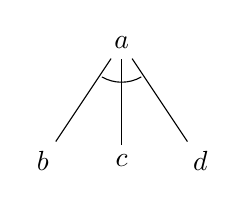
\begin{tikzpicture}
\node (v2) at (-0.5,1) {$a$};
\node (v1) at (-1.5,-0.5) {$b$};
\node (v4) at (-0.5,-0.5) {$c$};
\node (v3) at (0.5,-0.5) {$d$};
\draw (v1) -- (v2) -- (v3);
\draw (v4) -- (v2);
\draw (-0.25,0.567) arc (-59.9993:-120:0.5);
\end{tikzpicture} & \mpb[.6]
Für die Anfrage \lstinline$a(X)$ werden die Zeilziele \lstinline$b(X)$, \lstinline$c(X)$, \lstinline$d(X)$ erzeugt, die alle wahr sein müssen.
\mpe
\end{tabular}\\
Oder-Verknüfung: \lstinline$a(X) :- b(X) ; c(X) ; d(X).$\\
\begin{tabular}{L{.3} L{.7}}
\begin{tikzpicture}
\node (v2) at (-0.5,1) {$a$};
\node (v1) at (-1.5,-0.5) {$b$};
\node (v4) at (-0.5,-0.5) {$c$};
\node (v3) at (0.5,-0.5) {$d$};
\draw (v1) -- (v2) -- (v3);
\draw (v4) -- (v2);
\end{tikzpicture} & \mpb[.6]
Hier muss eines der Teilziele wahr sein.
\mpe
\end{tabular}

\cparagraph{Beispiel} Programm von oben:
\begin{center}
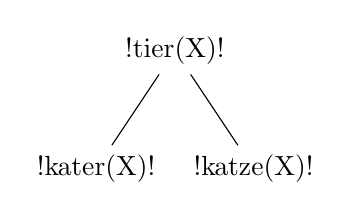
\begin{tikzpicture}
\node (v2) at (-0.5,1) {\lstinline!tier(X)!};
\node (v1) at (-1.5,-0.5) {\lstinline!kater(X)!};
\node (v3) at (0.5,-0.5) {\lstinline!katze(X)!};
\draw (v1) -- (v2) -- (v3);
\end{tikzpicture}
\end{center}
Bei der Anfrage \lstinline$tier(X)$ wird die Variable \lstinline$X$ ersetzt durch die Konstante \lstinline$reni$ und die Variablen auf tieferen Ebenen werden entsprechend ersetzt.\\
Schreibweise: \lstinline$X/reni$ (\lstinline$X$ wird unifiziert mit \lstinline$reni$)
\begin{center}
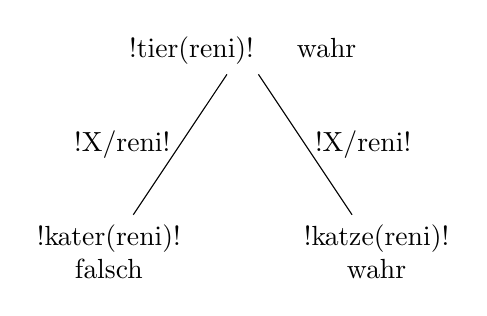
\begin{tikzpicture}[scale=1.7]
\node (v2) at (-0.5,1) {\lstinline!tier(reni)! ~~ wahr};
\node[align=center] (v1) at (-1.5,-0.5) {\lstinline!kater(reni)!\\ falsch};
\node[align=center] (v3) at (0.5,-0.5) {\lstinline!katze(reni)!\\ wahr};
\draw (v1) -- node[left]{\lstinline!X/reni!} (v2) -- node[right]{\lstinline!X/reni!} (v3);
\end{tikzpicture}
\end{center}
Allgemein kann ein Und-Oder-Baum aus beliebig vielen Und- oder Oder-Verknüpfungen bestehen.\\
Dieser Baum muss systematisch durchsucht werden, um einen Wahrheitswert für die Wurzel zu bestimmen.\\
Mögliche Strategien: Tiefensuche, Breitensuche.
\subsection{Tiefensuche}
Problem bei der Tiefensuche:
\cparagraph{Beispiel} $ $
\begin{lstlisting}[language=Prolog]
zug(X,Y) :- zug (Y,X).
zug(1,2).
\end{lstlisting}
Anfrage \lstinline$zug(2,1)$:
\begin{center}
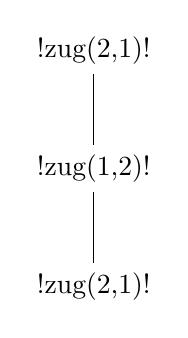
\begin{tikzpicture}
\node (v1) at (0,3.5) {\lstinline!zug(2,1)!};
\node (v2) at (0,2) {\lstinline!zug(1,2)!};
\node (v3) at (0,0.5) {\lstinline!zug(2,1)!};
\draw (v1) -- (v2) -- (v3);
\end{tikzpicture}
\end{center}
Der Und-Oder-Baum ist unendlich und eine Tiefensuche, die den ersten Zweig (links) verfolgt, findet keine Lösung.\\
Das gleiche Problem tritt bei einer entsprechenden Implementierung in Java auf:
\begin{lstlisting}[language=Java]
Boolean zug(int x, int y) {
	return zug(y,x) || (x==1 && y==2);
}
\end{lstlisting}
Die Breitensuche würde hier eine Lösung finden:
\begin{center}
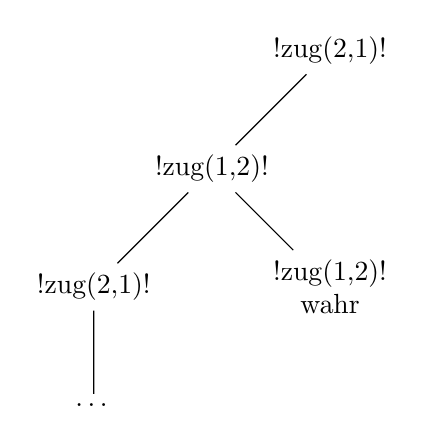
\begin{tikzpicture}
\node (v0) at (0,1.5) {\lstinline!zug(2,1)!};
\node (v3) at (-1.5,0) {\lstinline!zug(1,2)!};
\node (v2) at (-3,-1.5) {\lstinline!zug(2,1)!};
\node [align=center] (v4) at (0,-1.5) {\lstinline!zug(1,2)!\\ wahr};
\node (v1) at (-3,-3) {…};
\draw (v1) -- (v2) -- (v3) -- (v0);
\draw (v3) -- (v4);
\end{tikzpicture}
\end{center}
Das heißt, die Breitensuche liefert eine Lösung, die Tiefensuche unter Umständen nicht.\bigskip\\
Lösung: Die Abbruchbedingung der Rekursion muss die erste Klausel sein damit die Rekursion nicht endlos läuft bzw. die Tiefensuche die Abzweigung nimmt, die zu einer Lösung führt:
\begin{lstlisting}[language=Prolog]
zug(1,2).
zug(X,Y) :- zug(Y,X).
\end{lstlisting}




